\graphicspath{{chapters/09/images}}
\chapter{Gradient methods}

\section{Introduction}
When the model needs to integrate to find an ODE solution, the output is points in that integrated function.
$f$ and $f'$ are not known of the optimization problem, so a numerical approximation is needed.
The idea of gradient methods is to set $f'=0$.
Gradient methods can be applied to both constraint and unconstrained models.
Integrating constraints the problem becomes:

$$\begin{cases}\max f(x) &  \\ g_i(x)=0, & i \in \mathcal{I} \\ x \in \mathbb{R}^N &\end{cases}$$

Let $\mathcal{I}= 1,...,m$.
The traditional way to solve this problem is to translate this system to another function.
The Lagrangian function is used to take into account the constraints.

  \subsection{Lagrangian function}
  A Lagrangian function is defined as the function:

  $$L: \mathbb{R}^n \times \mathbb{R}^m \rightarrow \mathbb{R}$$

  Such that:

  $$L(x)= f(x) + \lambda g(x) = f(x) + \sum_{j=1}^m \lambda_j g_j(x)$$

  \subsection{Lagrangian Multipliers Theorem}
  If $x^*$ is a stationary point for a Lagrangian function, then $\exists \lambda^*$ such that $x^* \lambda^*$ is a stationary point for $L$.
  This is a necessary condition that increases the dimensionality of the problem to $\mathbb{R}^N \rightarrow \mathbb{R}^N \times \mathbb{R}^m$, but it allows to search solutions using the stationary points.
  This can be generalized to $g_i(x)\leq 0$ constraints.
  Stationary points are not necessarily minima and maxima.
  This is enforced by checking through second derivations or evaluating the function in other points.

  \subsection{Definition of a gradient}
  Let $f: \mathbb{R}^N \rightarrow \mathbb{R}$ a differentiable function, the gradient of $f$ is:

  $$\nabla f: \mathbb{R}^N \rightarrow \mathbb{R}^N$$

  Where:

  $$\nabla f_i=\frac{\partial}{\partial x_i} f(x)_i$$

  And:

  $$\nabla f(x) =\left[\begin{array}{c}\frac{\partial}{\partial x_1} f(x) \\ \vdots \\ \frac{y}{\partial x_N} f(x)\end{array}\right]$$

  The objective is looking for points for which the derivative vanishes:

  $$x^* : \nabla f(x^*)=0$$

    \subsubsection{Some examples}
    Two functions used to test optimization algorithms are the Rosenbrock's function:

    $$f(x, y)=(1-x)^2+100\left(y-x^2\right)^2$$

    And the Eggholder function:

    $$f(x, y)=-(y+47) \sin \left(\sqrt{\left.\mid \frac{x}{2}+(y+47)\right|}-\right. x \cdot \sin \left(\sqrt{\left.\mid x-(y+47\right)|}\right)$$

      Which are used to test optimization algorithms.
      Solving analytically these two problems is hard, so a numerical solution has to be employed.

  \subsection{Limitations of gradient descent methods}
  One of the major limitations of these algorithms is that there is no guarantee to reach the global minimum.
  Furthermore it could be the case that variables cannot be optimized together, so there is a need to make a trade-off between them.
  Finally gradient methods cannot be applied to stochastic simulations as their functions are not continuous.

  \begin{figure}[H]
    \centering
    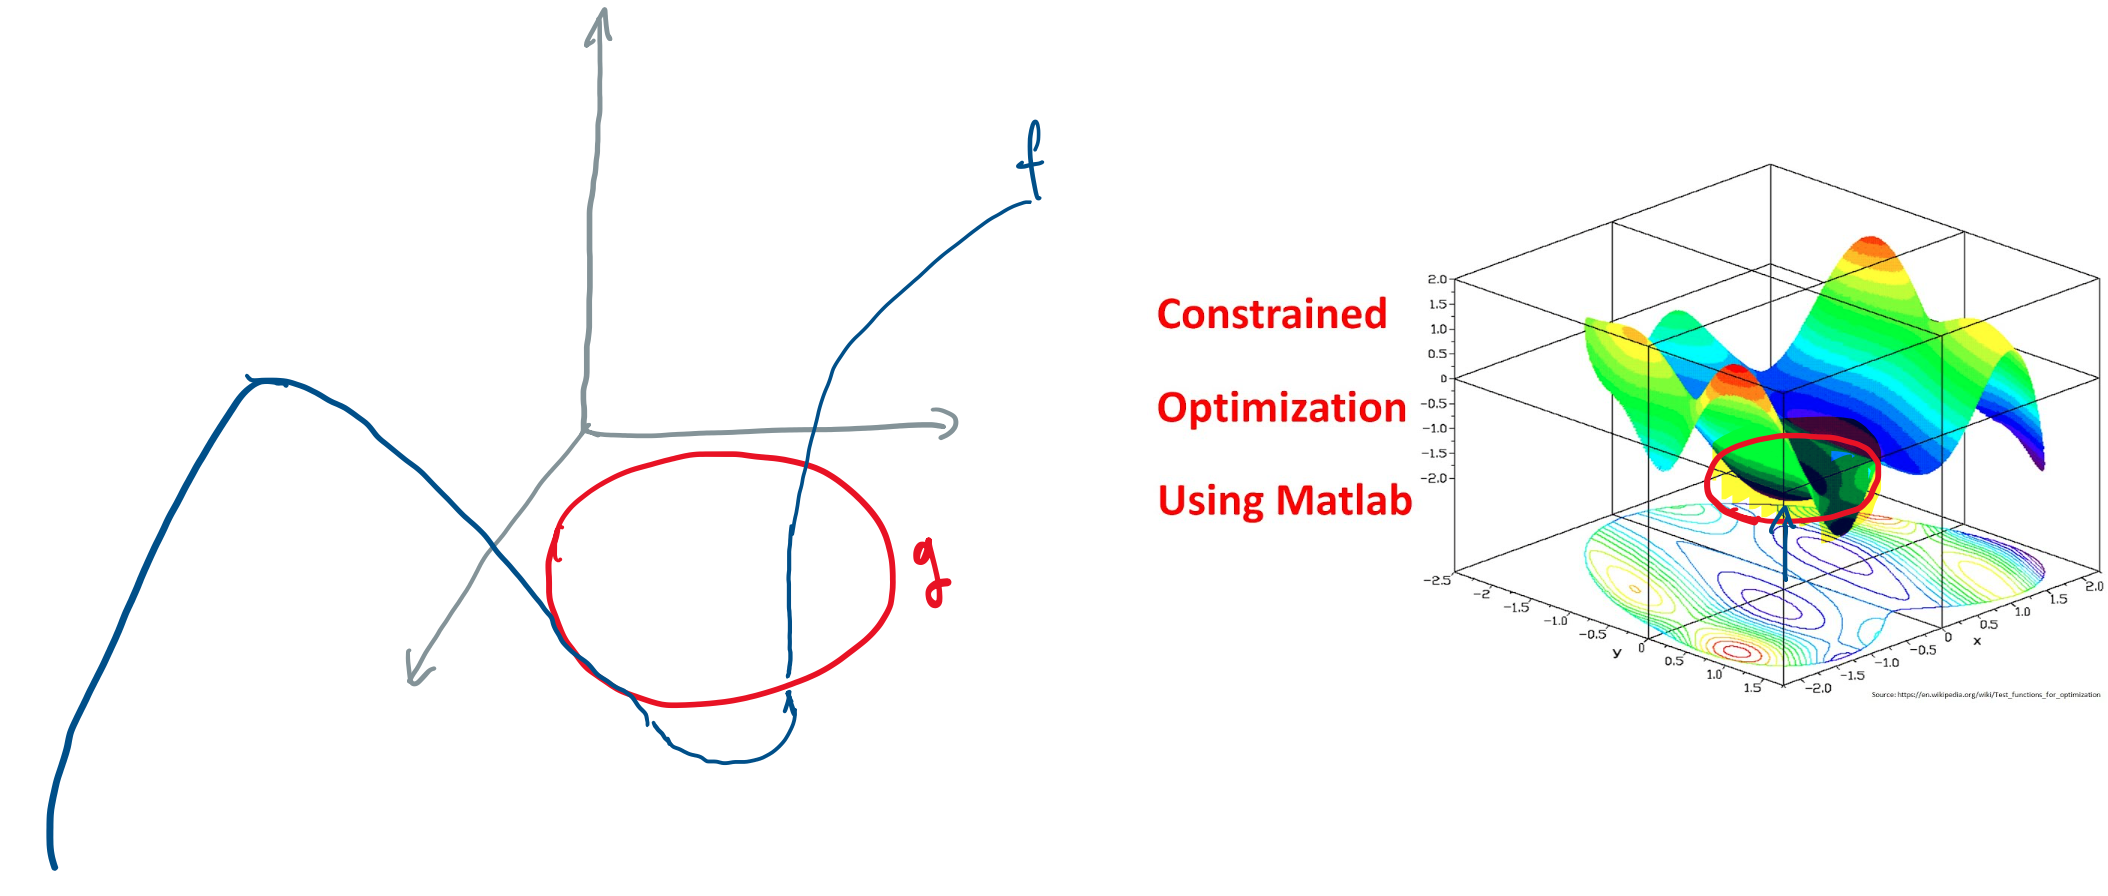
\includegraphics[width=0.5\textwidth]{example.png}
    \caption{Blue = function, red = constraint}
    \label{fig:ex}
  \end{figure}

  Figure \ref{fig:ex} is an example of an objective function.
  If there is an equality constraint only the points meeting the boundary, in red, are to be considered.
  In an inequality constraint instead everything inside the red circle is considered.
  Generally constraints reduce the search space: the Lagrangian determines that the minimum point with some multipliers will give a solution of the Lagrangian.
  Finding the solution of the original condition.
  These could not be solutions of the original conditions, but they are ideal candidates that can be checked.
  To perform an evaluation of the distance the model should be integrated.
  This is computational expensive, so the measure of computation is the number of times the model has to be simulated per iteration.

\section{Gradient approximation with Taylor formula}
In most cases the gradient is unknown and it should be approximated using the Taylor formula.
Let $]a,b[ \in \mathbb{R}, x_0 \in ]a,b[$ and $f_i]a,b[ \rightarrow \mathbb{R}$ be differentiable $(n-1)$ times in $]a,b[$ and $f^{(n)}$ continuous in $x_0$.
Then let $x \in ]a,b[$:

$$f(x)=f\left(x_0\right)+f^{\prime}\left(x_0\right)\left(x-x_0\right)+f''(x_0)\frac{(x-x_0)^2}{2!}+ ...+ f^{(n)}(x_0)\frac{(x-x_0)^n}{n!} + R_n(x)$$

Such that:

$$\lim_{x \rightarrow x_0} \frac{R_n(x)}{(x-x_0)^n} =0$$

Focussing on the first terms:

$$f(x)=f\left(x_0\right)+f^{\prime}\left(x_0\right)\left(x-x_0\right)+R_2(x)=0$$

$$f^{\prime}\left(x_0\right)= \frac{f(x)-f(x_0)}{x-x_0}+\left(\frac{R_2(x)}{(x-x_0)}\right)=\frac{f(x)-f\left(x_0\right)}{x-x_0}+R_1(x)$$

This trick can be used for any $N>1$.
Now let $f: \mathbb{R}^N \rightarrow \mathbb{R}$ and $e_i=(0, \ldots, 0,1,0,\ldots,0)$.
Consider $x_1 x+\varepsilon e_i, x-\varepsilon e_i$ so that the gradient is being explored in one direction:

\begin{align*}
  f\left(x+\varepsilon e_i\right)&=f(x)+\varepsilon \frac{\partial f}{\partial x_i}(x)+\frac{1}{2} \varepsilon^2 \frac{\partial^2 f}{\partial x_i{ }^2}(x)+R_3(x) \\
  f\left(x-\varepsilon e_i\right)&=f(x)-\varepsilon \frac{\partial f}{\partial x_i}(x)+\frac{1}{2} \varepsilon^2 \frac{\partial^2 f}{\partial x_i{ }^2}(x)+R_3(x) \\
  \Rightarrow f\left(x+\varepsilon e_i\right)-f\left(x-\varepsilon e_i\right)&=+2 \varepsilon \frac{\partial f}{\partial x_i}(x)+R_3(x) \\
  \Rightarrow \frac{\partial f}{\partial x_i}(x)&=\frac{f\left(x+\varepsilon e_i\right)-f\left(x-\varepsilon e_i\right)}{2 \varepsilon}+R_2(x)
\end{align*}

This is an approximation of the first derivative with improved accuracy.
This applies to only one derivative, so it has to be performed at least twice as $2$ function evaluation are needed for each $i\rightarrow 2W$.
In order to obtain a decent gradient, a lot of computations are required, but these are fust as they have a low number of iterations.
The algorithm converges when $\Delta f = 0$.

  \subsection{Vanishing gradient}
  There might be points where the gradient vanishes which are not the final destination.
  Gradient methods may tend to overfit, but they are effective.
  The main issue is that since the gradient is approximated, it cannot be trusted everywhere.
Gradient methods can be applied to two different categories of problems:

\section{Line search}
The line search is a class of algorithms that follow a direction along the gradient.


  \subsection{Newton's direction}
  Considering Taylor's formula and letting $x_k$ be the starting point, $\alpha \in \mathbb{R}^+$ the step length and $p$ the direction such that ($x_k, p \in R^n$).
  For $n=1$:

  $$
  f(x_k+\alpha p)=f(x_k) + \alpha p f'(x_k) + \frac{\alpha^2p^2}{2} f''(x_k) + r(p^3)
  $$
  For simplicity set $\alpha=1$ and truncate the formula:
  $$
  f(x_n+p)=f(x_n) + p f'(x_n) + \frac{p^2}{2} f''(x_n) = m_k(p)
  $$

  Now instead of $f$ the simple polynomial $m_k(p)$ is minimized.
  From this equation the direction $p = -\frac{f'(x_k)}{f''(x_k)}$ is obtained.
  This is Newton direction, which is the best direction to move the gradient.
  When $n>1$, $p = -(\nabla^2 f(x_k))^{-1}\nabla f(x_k)$.
  Finding the inverse of a matrix is not straightforward, so next algorithm will try to approximate it.
  The second derivative progressively shrinks when the algorithm approaches convergence to reduce the step size.

  \subsection{Line search algorithm for function minimization}
  An algorithm for line search for function minimization can be found in \ref{algo:line-search}.

  \begin{algorithm}[H]
\DontPrintSemicolon
\SetKwComment{comment}{$\%$}{}
\SetKw{Int}{int}
\SetKw{To}{to}
\SetKw{Return}{return}
\SetKw{Not}{not}
\SetKw{Input}{Input}
\SetKw{Output}{Output}
\SetKw{False}{false}
\SetKw{True}{true}
\SetKwData{Item}{item}
\SetKwFunction{Min}{min}
\SetKwFunction{Partitioning}{partitioning}
\SetKwFunction{TitleFunction}{Line search}

\caption{\protect\TitleFunction{}}
\label{algo:line-search}

\Input: the function $f$ to be minimized and $x_k$ starting point\;

\Output: the minimized function\;

\While{$||\nabla f(x_k)||>\epsilon$}{
	$p_k = -(\nabla^2 f(x_k))^{-1}\nabla f(x_k)$\;
	select $\alpha_k$\;
	$x_{k+1} = x_k+\alpha_kp_k = x_k-\alpha_k(\nabla^2f(x_k))^{-1}\nabla f(x_k)$\;
	$k = k+1$\;
}

\end{algorithm}


  The stopping point is when the gradient is equal to zero, but there is a need to apply a threshold $\epsilon$ on it.
  Now at each iteration sometimes approximation is needed to compute the inverse of the matrix.
  Moreover all these gradients are computationally expensive to compute.
  Nevertheless this process of going in one direction is smart.
  The smartest part, or the computation of $p_k$ can be approximated to make the computation less expensive.


  \subsection{Quasi Newton's direction}
  To avoid the computation of $\nabla^2 f$, a different matrix $B_k$ is built, such that

  $$B_{k+1}\cdot (x_{k+1}-x_k) = \nabla f(x_{k+1})-\nabla f(x_k)$$

  The second derivate is being approximated, the gradient is exploited to prevent extra computation.
  The Hessian where will not be computed.
  So the quasi-Newton direction will be:

  The fact that the second derivative progressively shrinks tells us that
  we need to reduce the step, but in this case we are not taking this into
  account. Of course we also have $\alpha$, we should look at Armijo
  condition and change it.
  Take into account that each time that we are performing operation on a
  number we lose precision.

  $$P_{k+1}=- \alpha B_{k+1}^{-1} \nabla f(x_k+1)$$


  \subsection{Steepest descent direction}
  In steepest descent the direction chosen is the one that reduces the gradient the most:

  $$p= -\alpha \frac{\nabla f}{||\nabla f||}$$

  The second derivative is being ignored and only the gradient computation is needed.
  This method converges more slowly with respect to Newton and Quasi Newton direction methods.

  \subsection{Selecting $\mathbf{\alpha}$}
  Ideally $\alpha$ should be defined such that:

  $$\bar{\alpha}= \arg \min_{\alpha>0} f(x_k+\alpha p)$$

  This is another optimization problem, which could be avoided by selecting an $\alpha$ such that:

  $$f(x_k+\alpha p) \leq f(x_k) + c_1\alpha \nabla f(x_n)^T p_k, c_1 \in (0,1)$$

  Such that the Armijio condition is satisfied: the reduction should be proportional to $\alpha$ and $\nabla f(x_n)^T p_k$.

  \subsubsection{Convergence of a method}
  The order of convergence of a method is a constant $\ell$, such that exists the limit:

  $$\lim_{k \rightarrow \infty  }\frac{||f(x_{k+1})-f(x^*)||}{||f(x_{k})-f(x^*)||^\ell} = L >0$$

  Where $x^*$ is the solution and the method converges.
  The new iteration is compared to the old one.
  The limit should go to $0$ and the exponent is the speed at which this happens: the higher $\ell$ the faster the numerator go to zero with the respect to the denominator, so the higher the exponent, the faster the convergence.
  For the methods discussed previously:

  \begin{multicols}{2}
    \begin{itemize}
      \item Steepest descent: $\ell=1$, linear convergence.
      \item Quasi-Newton: $\ell \in (1,2)$, superlinear convergence.
      \item Newton: $\ell=2$, quadratic convergence.
    \end{itemize}
  \end{multicols}


\section{Trust region}
Trust region is a class of algorithms that create an approximation of the problem and they solve it in a small trustable region.

{[}picture{]}
\noindent
Imagine that this is a cut function: the starting point $x_k$ is in the middle.
The main idea of the trust region is that a direction is not followed: the function is approximated  with a simpler function like through Taylor approximation.
According to how big and reliable the approximation is, a direction is chosen.
The model can be approximated as:

$$m(x_p+\alpha p)=f(x_k)+\alpha p^T \nabla f(x_k)+ \frac{1}{2} \alpha^2p^T B_k p$$

$$\alpha=1, m_k (p)=f_k+p^T\nabla f_k + \frac{1}{2} p^T B_k p$$

  \subsection{Trust region steepest descent}
  In trust region steepest descent a region is defined such that $||p|| < \delta_k,\delta_k>0$.
  The optimization problem will be solved in this region.
  $B_k$ can be the Hessian matrix or an approximation, but it can also be ignored.
  Finding a minimum for $m_k(p)=f_k+p^T\nabla f_k$ means that the objective is:

  $$\min_p m_k(p)= \min_p (f_k+p^T\nabla f_k)$$

  $f_k$ is a constant, so a direction for which $\min_p p^T\nabla f_k$ is minimum.
  The problem can be re-written as:

  $$p^T\nabla f_k = ||p|| ||\nabla f_k|| \cos \theta$$

  Now the procedure is to minimize for $p$ such that $\cos \theta = -1$ and $||p||=\delta_k$,
  where $||p|| \leq \delta_k$ is the radius of the trust region.

  $$\min_p p^T\nabla f_k = -\delta_k || \nabla f_k ||$$

  $$p = - \delta_k \frac{\nabla f_k}{||\nabla f_k||}$$

  This result is exactly the equation from steepest descent.
  A condition on the region with $\delta_k$ is being applied.
  This direction and the whole approach is called trust region steepest descent.
  The same idea could be followed by applying Newton or Quasi-Newton.

  \subsection{Evaluating the trust regions}
  To evaluate the trust regions, the actual reduction is defined as:

  $$\rho_k = \frac{f(x_k)-f(x_k+p)}{m(x_k)-m(x_k+p)}$$

  By construction $m(x_k+p) \leq m(x_k)$.

  \begin{multicols}{2}
    \begin{itemize}
      \item If $\rho_k < 0$, reject $p$, as the real problem is not being improved.
      \item If $\rho_k \simeq 1$ a maybe longer step can be considered.
    \end{itemize}
  \end{multicols}
  Usually take $\delta_k = \frac{1}{4} \delta_k$
  The value of $\delta$ can be tuned according to the needs of the problem.
  The approach is similar to  the RK method.
  A grey area  between $0$ and $1$ is found, so a threshold is defined such that $\rho_k < \eta$ and$\rho_k > \eta$.


  \subsection{Trust region algorithm}
  An implementation of the trust region method is outlined in algorithm \ref{algo:trust-region}.

  \begin{algorithm}[H]
\DontPrintSemicolon
\SetKwComment{comment}{$\%$}{}
\SetKw{Int}{int}
\SetKw{To}{to}
\SetKw{Return}{return}
\SetKw{Not}{not}
\SetKw{Input}{Input}
\SetKw{Output}{Output}
\SetKw{False}{false}
\SetKw{True}{true}
\SetKwData{Item}{item}
\SetKwFunction{Min}{min}
\SetKwFunction{Partitioning}{partitioning}
\SetKwFunction{TitleFunction}{Trust region}

\caption{\protect\TitleFunction{}}
\label{algo:trust-region}

\Input: the function $f$ to be minimized and $x_k$ starting point, $\delta$ and $\eta$ parameters\;

\Output: the minimized function\;

$\delta>0$\;
$\delta_0\in]0,\delta[$\;
$\eta \in\biggr]0,\frac{1}{4}\biggr[$\;
$k = 0$\;
$\epsilon < 0$\;

\Repeat{$||\nabla f(x_k)||<0$}{
	obtain $p_k$ such that $p_k=\arg\min\limits_{p}m(x_k+p)$\;
	compute $p_k$\;
	\If{$\rho_k<\frac{1}{4}$}{
		$\delta_{k+1} = \frac{1}{4}\delta_k$\;
	}
	\ElseIf{$\rho_k < \frac{3}{4}\land||p_k||=\delta_k$}{
		$\delta_{k+1} = \min(2\delta_k, \hat{\delta})$\;
	}
	\Else{
		$\delta_{k+1} = \delta_k$\;
	}
	\If{$\rho_k >\eta$}{
		$x_{k+1} = x_k +p_k$\;
	}
	\Else{
		$x_{k+1} = x_k$\;
	}
}

\end{algorithm}


  The stopping point is when the gradient is sufficiently small.
  The focus is on computing $p_k$, then $\rho_k$ is evaluated to adjust the parameters.
